% ch06-bitemporal-grid.tex — 2D Bitemporal Coordinate Grid (VI edition)
% X = Valid Time (Thời gian hiệu lực); Y = Transaction/System Time (Thời gian hệ thống)
% Coordinates scaled: x = year-2016, y = year-2018 (2016..2026 -> 0..10).
% Claim C1: valid [2018,2024), tx [2020,2024), range [300K,450K]
% Claim C2: valid [2022,2026+), tx [2024,2026+), range [300K,400K]
\documentclass[tikz,border=5pt]{standalone}
\usepackage{fontspec}
\setmainfont{Times New Roman}
\usepackage{unicode-math}
\setmathfont{Cambria Math}
\usetikzlibrary{patterns,positioning,fit,arrows.meta,calc}

\begin{document}
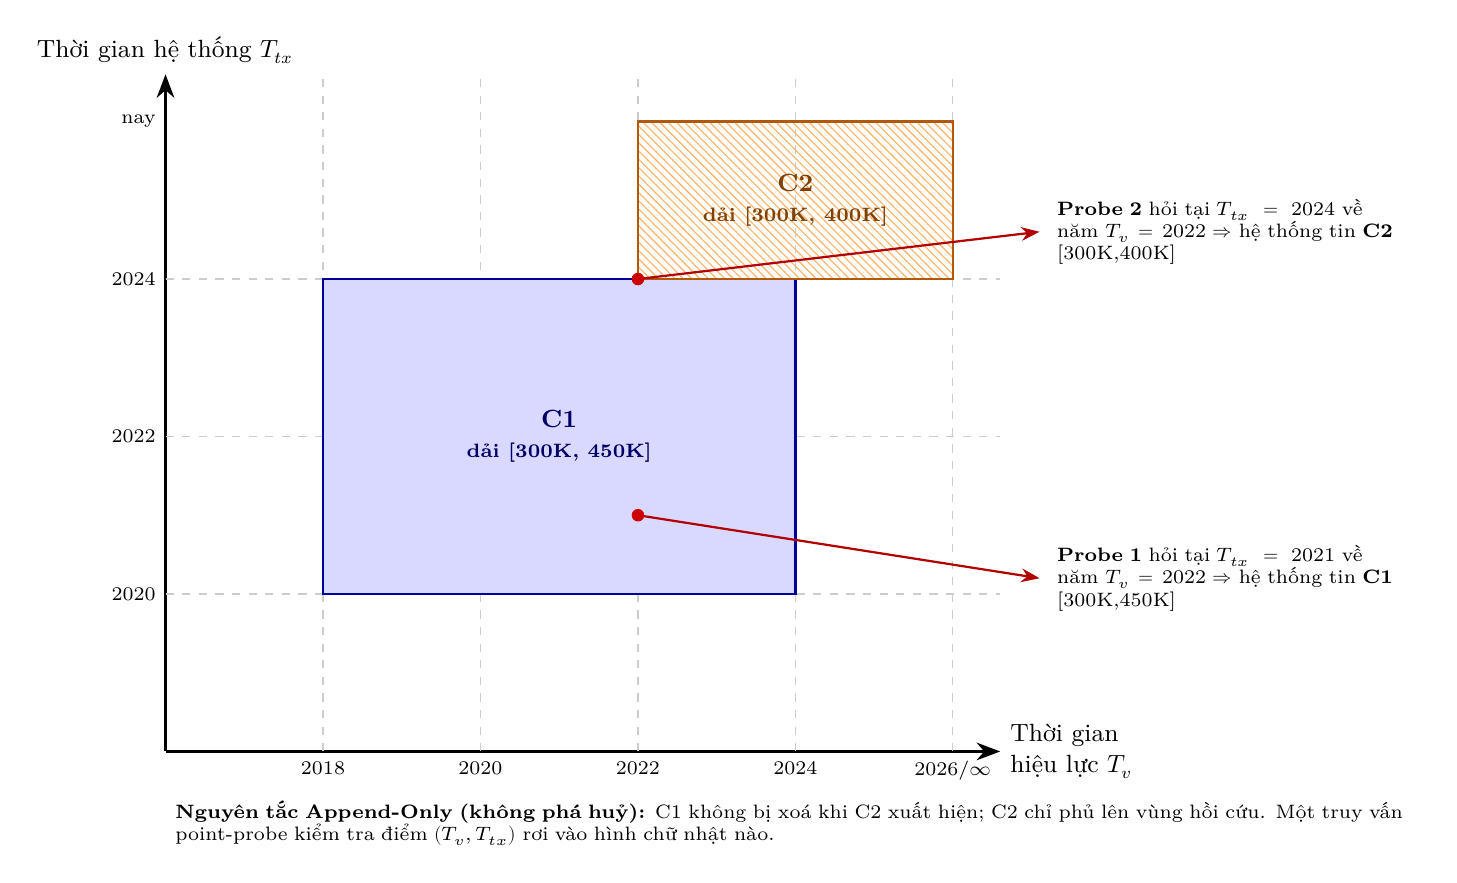
\begin{tikzpicture}[
    axis/.style={thick, -{Stealth[length=3mm]}},
    gridline/.style={thin, gray!40, dashed},
    boxlabel/.style={font=\small\bfseries, align=center},
    probelabel/.style={font=\scriptsize, align=left, text width=4.6cm},
    probe/.style={circle, fill=red!80!black, inner sep=1.6pt, outer sep=0pt},
    leader/.style={->, >=Stealth, red!70!black, thick},
]

\def\xmin{0}  \def\xmax{10.6}
\def\ymin{0}  \def\ymax{8.6}

% Axes
\draw[axis] (\xmin, \ymin) -- (\xmax, \ymin) node[right, font=\small, align=left] {Thời gian\\hiệu lực $T_v$};
\draw[axis] (\xmin, \ymin) -- (\xmin, \ymax) node[above, font=\small, align=center] {Thời gian hệ thống $T_{tx}$};

% Vertical grid + X ticks
\foreach \yr in {2018,2020,2022,2024} {
    \pgfmathsetmacro{\gx}{\yr-2016}
    \draw[gridline] (\gx, \ymin) -- (\gx, \ymax);
    \node[font=\scriptsize, below] at (\gx, \ymin) {\yr};
}
\draw[gridline] (10, \ymin) -- (10, \ymax);
\node[font=\scriptsize, below] at (10, \ymin) {2026/$\infty$};

% Horizontal grid + Y ticks
\foreach \yr in {2020,2022,2024} {
    \pgfmathsetmacro{\gy}{\yr-2018}
    \draw[gridline] (\xmin, \gy) -- (\xmax, \gy);
    \node[font=\scriptsize, left] at (\xmin, \gy) {\yr};
}
\node[font=\scriptsize, left] at (\xmin, 8) {nay};

% Claim C1: (2,2) to (8,6)
\fill[blue!15] (2,2) rectangle (8,6);
\draw[blue!60!black, thick] (2,2) rectangle (8,6);
\node[boxlabel, blue!40!black] at (5,4) {C1\\{\scriptsize dải [300K, 450K]}};

% Claim C2: (6,6) to (10,8)
\fill[orange!20, pattern=north west lines, pattern color=orange!60] (6,6) rectangle (10,8);
\draw[orange!70!black, thick] (6,6) rectangle (10,8);
\node[boxlabel, orange!50!black] at (8,7) {C2\\{\scriptsize dải [300K, 400K]}};

% Probe 1: (Tv=2022, Ttx=2021) -> (6,3) inside C1; label in right margin
\node[probe] (p1) at (6,3) {};
\draw[leader] (p1) -- (11.1, 2.2);
\node[probelabel, anchor=west] at (11.2, 2.2) {\textbf{Probe 1} hỏi tại $T_{tx}=2021$ về năm $T_v=2022$ $\Rightarrow$ hệ thống tin \textbf{C1} [300K,450K]};

% Probe 2: (Tv=2022, Ttx=2024) -> (6,6) inside C2; label in right margin
\node[probe] (p2) at (6,6) {};
\draw[leader] (p2) -- (11.1, 6.6);
\node[probelabel, anchor=west] at (11.2, 6.6) {\textbf{Probe 2} hỏi tại $T_{tx}=2024$ về năm $T_v=2022$ $\Rightarrow$ hệ thống tin \textbf{C2} [300K,400K]};

% Append-only / non-destructive note (below the plot)
\node[anchor=north west, font=\scriptsize, text width=15.6cm, yshift=-0.35cm] at (0, -0.15) {\textbf{Nguyên tắc Append-Only (không phá huỷ):} C1 không bị xoá khi C2 xuất hiện; C2 chỉ phủ lên vùng hồi cứu. Một truy vấn point-probe kiểm tra điểm $(T_v, T_{tx})$ rơi vào hình chữ nhật nào.};

\end{tikzpicture}
\end{document}
